\documentclass[conference]{IEEEtran}
%\usepackage[backend=biber,style=authoryear]{biblatex}
%\addbibresource{bibliography.bib}
\usepackage{hyperref}
\usepackage{amsmath}
\usepackage{amsfonts}
\usepackage{amssymb}
\usepackage{float}
\usepackage{graphicx}
\usepackage{booktabs}
\usepackage{array}
\title{Evaluating Query Performance Between Relational and Graph Databases Using Neo4j and MySQL}
\author{\IEEEauthorblockN{David Josephs}
	\IEEEauthorblockA{\small Southern Methodist University\\
	Dallas, Texas\\
	Email: josephsd@smu.edu}
	\and
	\IEEEauthorblockN{Samantha Sprague}
	\IEEEauthorblockA{\small Southern Methodist University\\
	Dallas, Texas\\
	Email: ssprague@smu.edu }
	\and
	\IEEEauthorblockN{Carson Drake}
	\IEEEauthorblockA{\small Southern Methodist University\\
	Dallas, Texas\\
	Email: drakec@smu.edu}

}
\date{\today}

\begin{document}
\maketitle
\begin{abstract}
    The popularity of graph databases has risen as the need to glean complex insights from diverse and large data sets multiplies. Historically,  relational databases have dominated the market share due to application performance requirements. With advances in machine learning and artificial intelligence, the ability to turn action into insights is critical in product success. This capability requires the ability to manage sophisticated relationships. The surge of graph databases and big, connected data comes with two big questions: do graph databases have the performance necessary to be implemented in applications, and do relational databases have the ability to properly model these intricate relationships?
\end{abstract}
\section{Introduction}
We intend to evaluate the relative performance between relational databases and graph databases with respect to latency (MS) and database size (GB). In this report, the relational database chosen was MySQL and the graph database chosen was Neo4j. The databases were evaluated using the same data set, in order to measure performance in different operations and queries.

\subsection{Background}
The primary difference between relational and graph databases is that in a relational database, the relationships are defined at a higher level, in the table definitions, while in a graphical database the relationships are defined in records. This means that a graph database may be more flexible and fluid in structure, which bears certain advantages and disadvantages over the relational model.

A relational database should be capable of querying massive amounts of records faster, as the structure of the data is pre-defined, whereas a graph database has to read each individual record to determine the structure. Similarly, because the relationships are not stored in the tables of a relational database, the relational database should take up less storage space. However, a graph database has a few key advantages over the relational database. When trying to perform path operations in a relational database (for example, if the data set contains info on Hollywood actors, finding co stars of co stars of an actor), the user has to recursively perform a huge set of joins, which causes memory usage and query latency to skyrocket. A graph database does not have these issues, as the connection between individual data points are defined within the data. That is, query latency and memory usage are not proportional to how much of the data the user chooses to explore (and the length of the path), but to the actual size of the data. Similarly, when finding a friend-of-friends or co-star-of-co-star relationship, a graph database should have a much simpler query structure.
\subsection{Neo4j}
Neo4j is an ACID compliant, transnational, NoSQL graph database. Technically, it is a \emph{native graph database}, which means that the graph model is implemented on all levels of the database, down to data storage. The database uses pointers to navigate the user-defined graph\cite{neo4jdef}.

Neo4j specifically follows the \emph{property graph model} which consists of \emph{nodes} and \emph{relationships}. The nodes populate the graph, containing attributes, known as properties (analogous to tables in a relational model). Nodes can be labelled in order to define their role in the model, as well as to define meta data. Relationships provide direct connections between nodes, and also contain attributes, known again as properties. An example of nodes and relationships is seen in \autoref{fig:noderel}
\begin{figure}[h]
   \centering
  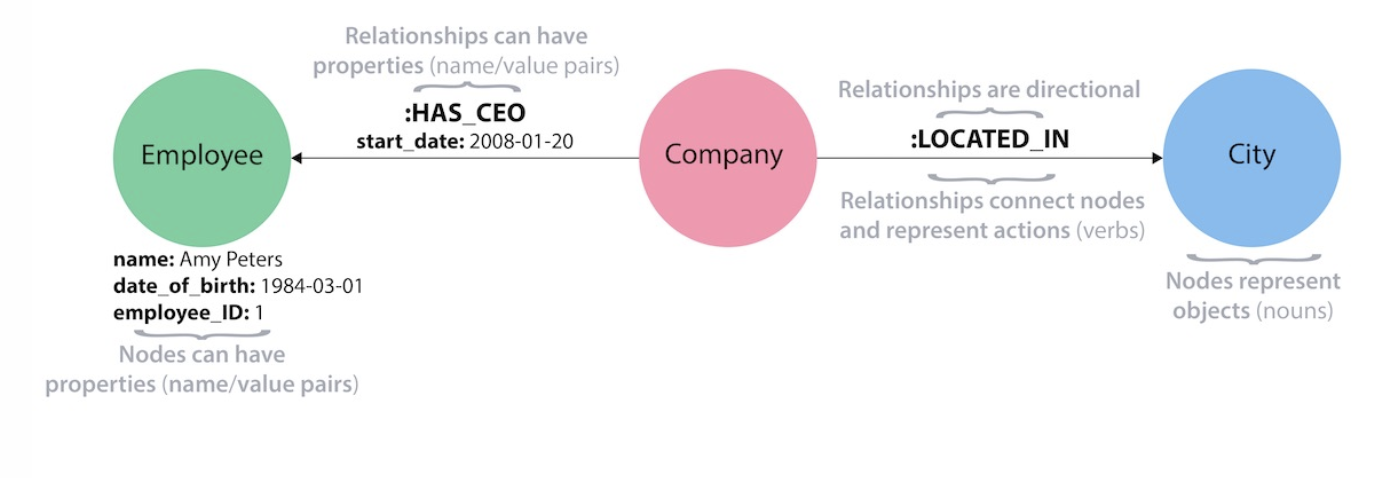
\includegraphics[scale=.4]{noderel.png}
 \caption{The property graph model}
\label{fig:noderel}
\end{figure}
\cite{neo4jdef}

Neo4j is currently a hot topic in graph databases, ran by companies from tech giants like Adobe and Microsoft to social media sites such as LinkedIn, and others such as the US Army and Volvo.
\subsection{MySQL}
We provide some background on MySQL. MySQL is blah blah blah

\subsection{Literature Review}
In \cite{kirby2014comparison}, Neo4j and MariaDB were tested on support and storage and querying linked graphs, in which Neo4j outperformed MariaDB in terms of storage, speed, and ease of use. In \cite{vicknair2010comparison} Neo4j and MySQL were compared in terms of objective benchmark tests and in different types of queries. Overall, it was found that the graph database performed better at at structural and full-text character queries, and worse on numerical queries. In \cite{marko2011comparison} MySQL and Neo4j are used to compare the differences in performance looking at large scale graph traversal using an artificial data set. In \cite{pandey2018comparison}, researchers looked at comparisons between a relational database (MySQL), a graph database (Neo4j), and a document store database (MongoDB) while assessing vehicle transactions between a company and their customers. In \cite{martinez2016comparison}, MySQL and Neo4j were compared in the context of an application used for advanced cancer treatment, using twelve queries with 3 different data sizes. It was found that in most standard queries, MySQL performed overall better than Neo4j, however in queries which involve multiple joins, Neo4j outperformed MySQL.    
\section{Experimental Methods}
\subsection{Data Set}

In order to adequately compare two fundamentally different datasets, an appropriate dataset must be chosen. For the purpose of this study, the Northwind \cite{microsoft} dataset was selected. The Northwind database contains information on a fictional company which imports and trades food from around the world, and comes with the Microsoft Office suite \cite{nwindDef}.
The Northwind database is commonly used to train professionals in SQL and database administration, and thus is widely documented and studied. This means it makes a perfect, well-understood control group. As it is designed for experimentation, it provides the opportunity to execute and practice any sort of queries necessary for comparison 

\section{Procedure}
    This will be an observational study leveraging statistical methods: ANOVA, and t-tests to evaluate the differences in the means for both query latency and size across the two databases by data-type.

    The steps to properly conducing a statistical test include: defining the problem statement, hypothesis declaration, assumption evaluation, critical value, t-statistic, and p-value acknowledgment, and a thorough conclusion mentioning the type of experiment and the scope of the analysis.

    Details of the tests will be examined as the schemas are defined.

\subsection{Evaluation}
We will be evaluating each database on its query latency using both numeric
and string based indexes. A set of trials will be carried out for each index type. A trial will consist of twenty queries selecting all relations at six levels of separation (degrees separation from a random entity starting at zero). A total of 480 queries will be carried out.

\subsubsection{Numeric Index Queries}\label{numeric-eval}
Both databases will be carry out a trial of queries utilizing a purely numeric encoded keys. This will allow us to evaluate if the indexing engines for MySQL and Neo4j optimize indexes depending on data type.

\subsubsection{Sting Index Queries}
The same evaluation described in \ref{numeric-eval} will be repeated, except 
this trial will utilize string encoded keys.


\bibliographystyle{IEEEtran.bst}
\bibliography{bibliography.bib}    
\end{document}
